\subsection{Object similarity}
We now look at the similarity between image A and B. The results can be seen in \autoref{object}.

\begin{figure}
	\centering
	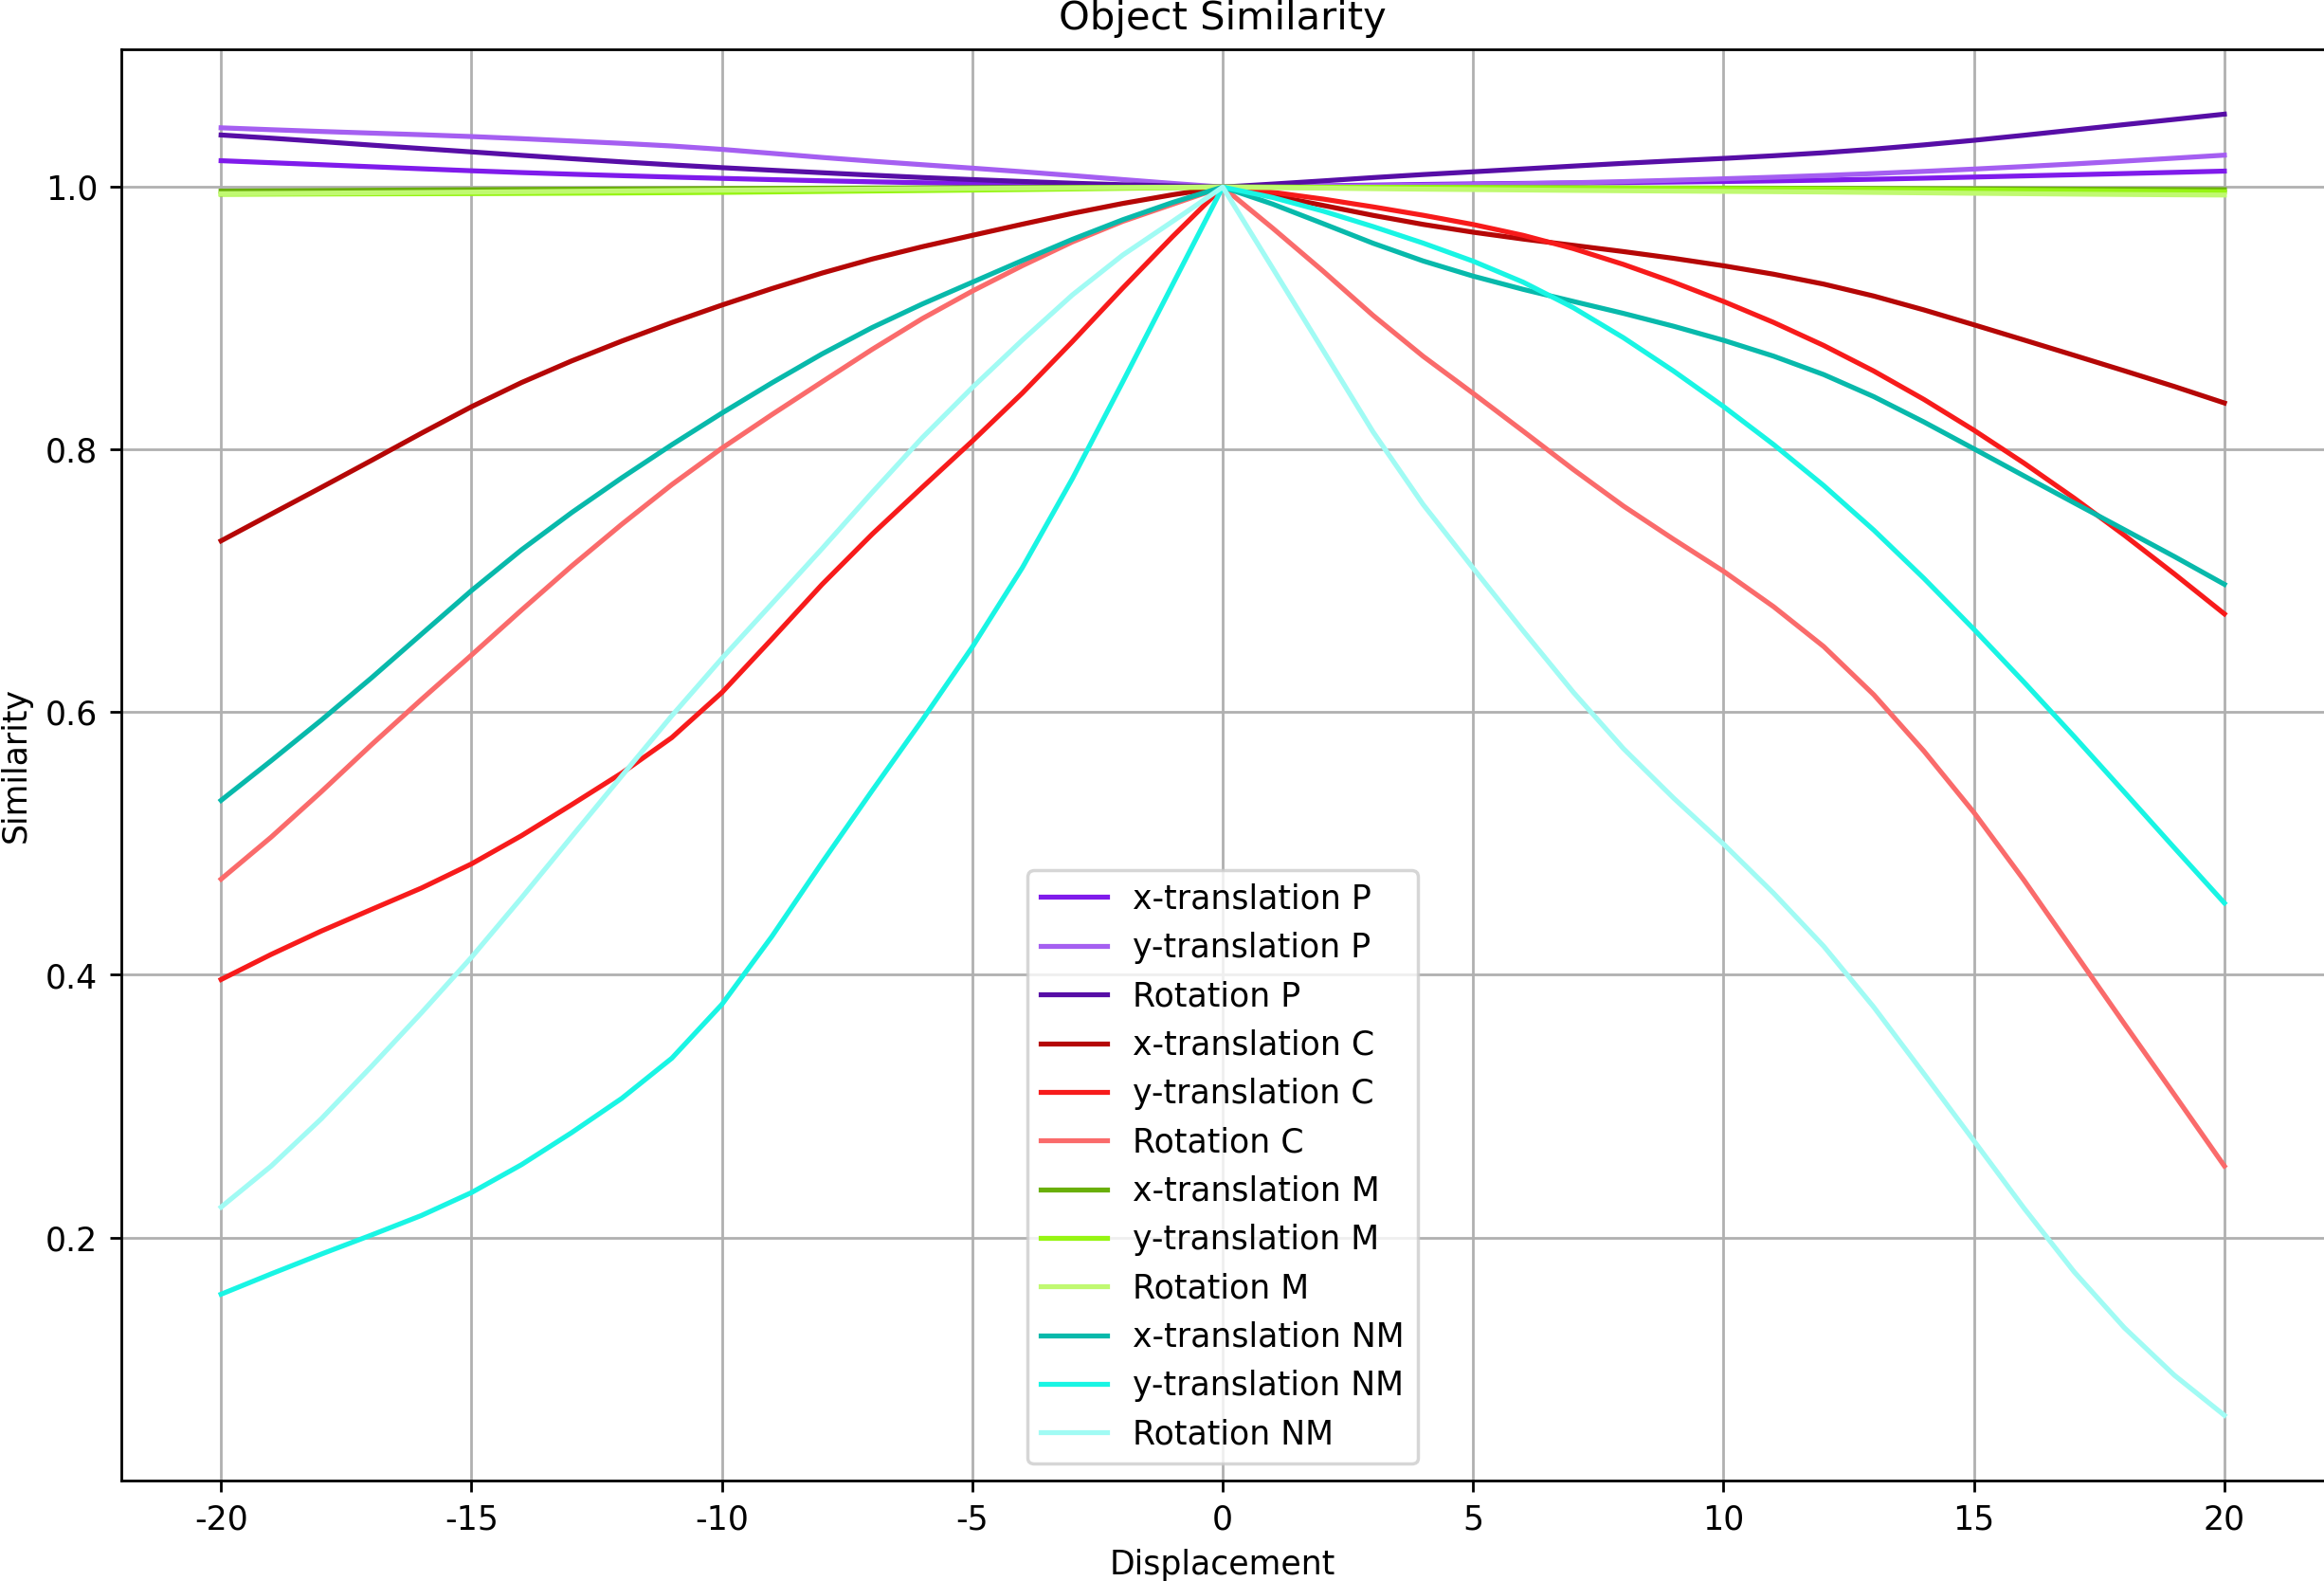
\includegraphics[width=0.8\linewidth]{Materials/objectSimilarity}
	\caption{Object similarity results normalized such that all optima touch 1.0. Both images have been blurred by a Gaussian kernel with sigma being 1. Translation displacement is measured in pixels and rotation displacement is measured in degrees. P = P-norm with P being 2, C = normalized cross correlation, M = mutual information, NM = normalized mutual information.}
	\label{object}
\end{figure}
We here see that all similarity measures again behaves correctly, however, compared to the self similarity results in \autopageref{self} the graphs have become more 'pointy' which would indicate the images are less similar as we need a smaller displacement to make the images dissimilar. By looking at the un-normalized similarity values it can also be reported that the similarity at optima has dropped for all similarity measure. However, we still see the optima being at 0 displacement. This might be due to the foreground and background being the most 'dominant' features in the images, and thus translating and rotating these out of the images might result in a bigger dissimilarity than aligning the images on the motif. We also see for NCC and NMI that the curves have become rather uneven / wavy and not as smooth as for self similarity. This is especially true around 1.0. The more wavy shapes of the curves could be an issue if we would like to optimize the functions with a gradient based method as the waves could form local minima and maxima. We see that the gradients of P-norm and MI is even more flat than for self similarity, making them hard to optimize. 